\documentclass{report}
\usepackage{hyperref}
\usepackage{graphicx}
\usepackage{enumerate}
\usepackage{enumitem}
\usepackage{xcolor}
\usepackage{import}
\usepackage{pdfpages}
\usepackage{microtype}


\usepackage{geometry}
 \geometry{
 left=1 in,
 right=1 in,
 bottom=1 in,
 top=1 in
}

\setlength\parindent{0pt}

\definecolor{lightGray}{HTML}{d8dde6}

\newcommand*{\backtrack}{\setcounter{enumi}{\numexpr\theenumi-1\relax}}

\title{\textbf{Scholastic Bowl} \\ Round 1 --- Set 3}
\author{Pranaav Sureshkumar \\ \href{mailto:pranaav2@illinois.edu}{pranaav2@illinois.edu}}
\date{\today}

\begin{document}

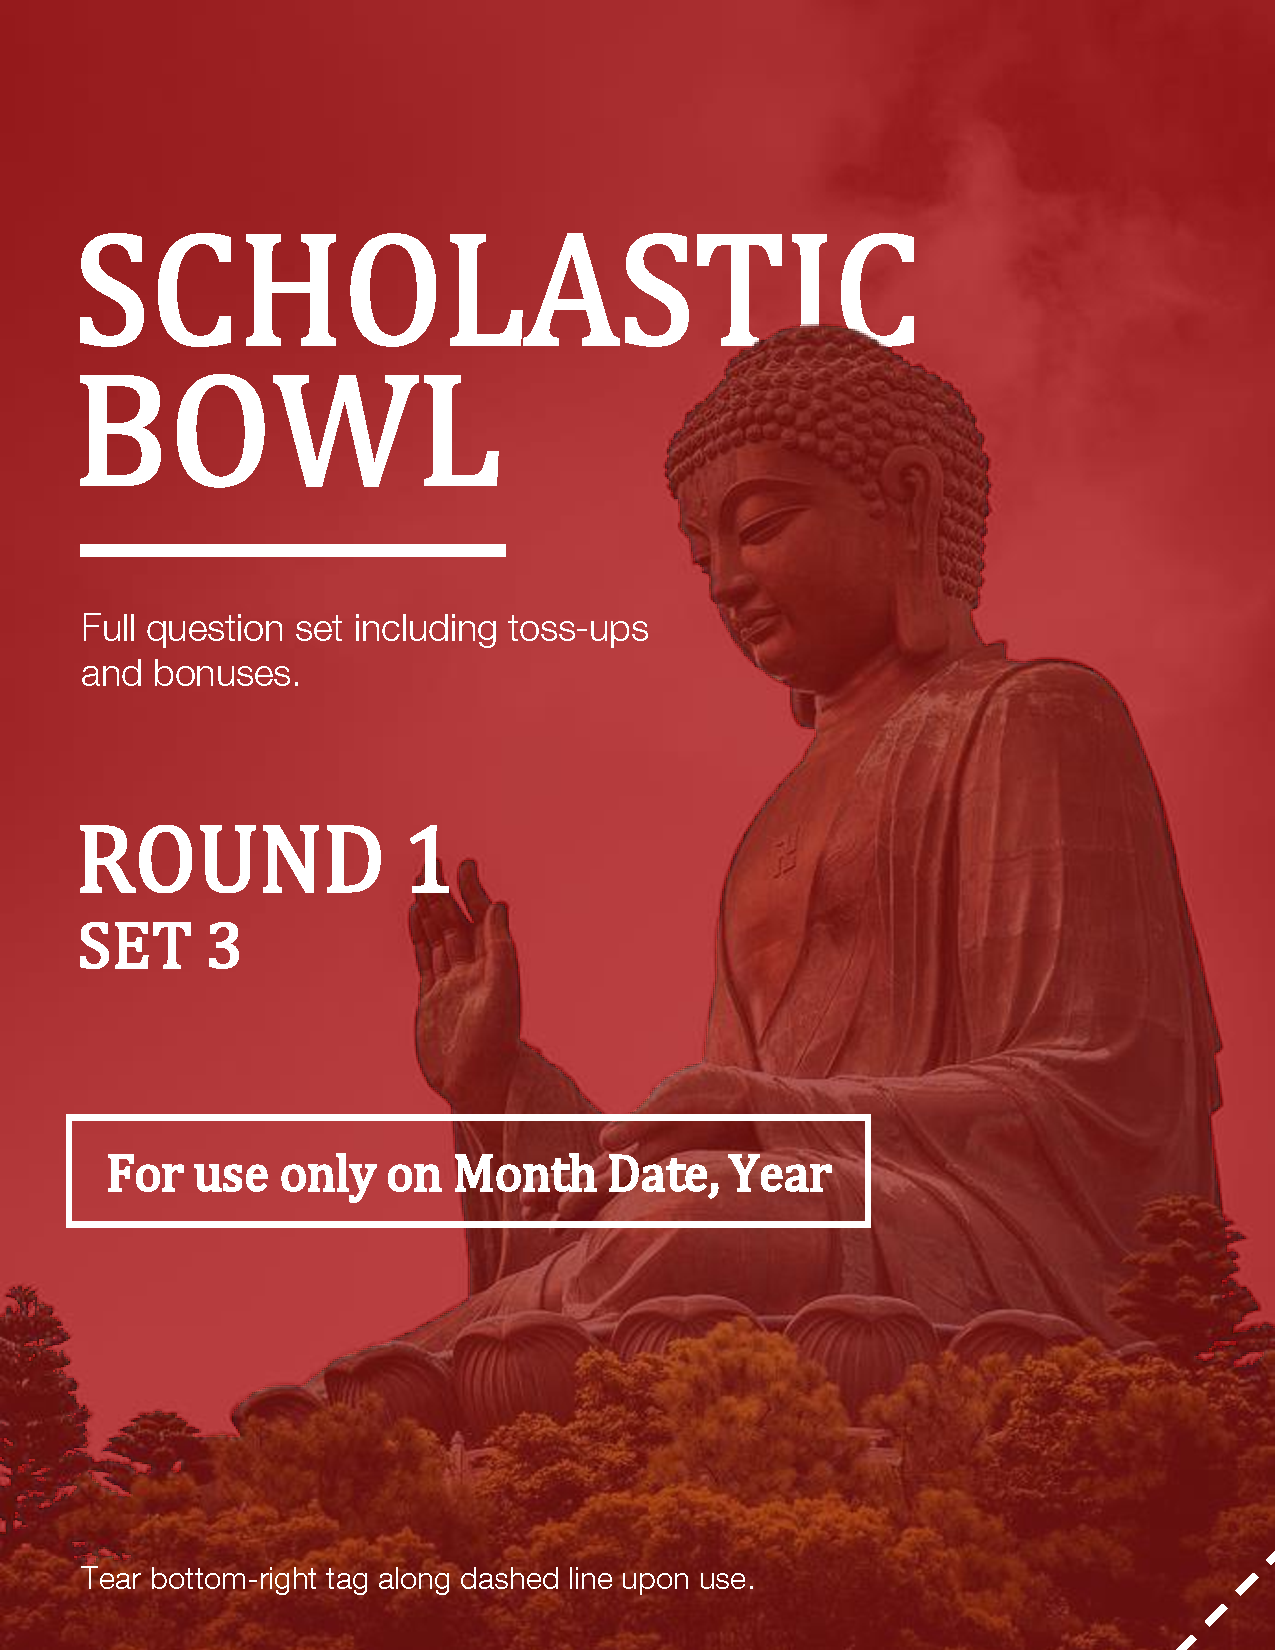
\includepdf[pages=-]{../Title Pages/Round 1 Set 3 Title Page.pdf}

\maketitle

\import{../Rules/}{Rules.tex}

\newpage

\vspace*{\fill}
\centering
\thispagestyle{empty}
\Large
Questions begin on the next page.
\vspace*{\fill}

\normalsize
\newpage
\setcounter{page}{1}

\begin{enumerate}
    % Question 1
    \item \textbf{HISTORY} \\ \textit{This} former Premier of the Soviet Union introduced a series of Five-Year Plans to collectivize agriculture and expand heavy industry. \textit{This} man supported Vladimir Lenin's Bolshevik party (*) and was a key proponent in the Russian Revolution. Upon Lenin's death, \textit{this} man defeated and banished Leon Trotsky to become leader of the USSR. For 10 points, name \textit{this} communist leader who led the Soviet Union in World War II. \\ ANSWER: Joseph \underline{Stalin} \backtrack
    \item \textbf{SCIENCE} \\ Black holes are regions of spacetime where a gravitational field is so strong that nothing can escape it. Name the following terms used to describe black holes by their definitions. For 10 points each,
    \begin{enumerate}[label=\Alph*]
        \item \textit{This} term, also called the \textit{point of no return}, is used to define the boundary of a black hole. If anything crosses \textit{this} boundary, it will inevitably be swallowed by the black hole. \\ ANSWER: \underline{event horizon}
        \item The largest type of black hole, like the one at the center of the Milky Way, is described by \textit{this} adjective. \\ ANSWER: \underline{supermassive}
        \item  The supermassive black hole at the center of the Milky Way is named \textit{this}. \\ ANSWER: \underline{Sagittarius A}*
    \end{enumerate}

    % Question 2
    \item \textbf{MISCELLANEOUS} \\ \textit{This} game’s soundtrack includes \textit{Subwoofer Lullaby} and \textit{Stal}, works by C418 \colorbox{lightGray}{[\textbf{See}\textperiodcentered ``four''\textperiodcentered ``eighteen'']}, whose songs can be found on in-game discs. In 2021, \textit{this} game added goats in an expansion that failed to update its (*) caves or cliffs. An enemy in \textit{this} game is the result of a coding error that turned what was supposed to be a pig into an elongated monster that becomes aggressive when looked at. For 10 points, name \textit{this} video game in which players build structures out of blocks until they’re blown up by creepers. \\ ANSWER: \underline{Minecraft} \backtrack
    \item \textbf{LITERATURE} \\ Answer the following questions about female Titans in Greek mythology. For 10 points each,
    \begin{enumerate}[label=\Alph*]
        \item Like later Greek gods, the Titans represented elements of the natural world. The Titaness Selene was the embodiment of \textit{this} natural satellite of Earth, which dominates the night sky. \\ ANSWER: \underline{moon}
        \item \textit{This} Titaness was the mother of the archer twins Apollo and Artemis. When the queen Niobe mocked \textit{this} Titaness for only having two children, Apollo and Artemis killed all of Niobe’s children. \\ ANSWER: \underline{Leto}
        \item \textit{This} Titaness was the Greek goddess of witchcraft. She was the handmaiden of Persephone and the goddess of ghosts. \\ ANSWER: \underline{Hecate}
    \end{enumerate}

    % Question 3
    \item \textbf{FINE ARTS} \\ \textit{This} musical work uses the melody of the folk song “At the Gate,” and it opens with the hymn “O Lord, Save thy People.” \textit{This} work’s composer hated his composition; he disliked its overt patriotism and felt it was too noisy, possibly because he orchestrated it with (*) cannons. \textit{This} work uses \textit{La Marseillaise} \colorbox{lightGray}{[La Mar\textperiodcentered ``say''\textperiodcentered\textbf{yez}]} to represent the invading French army, and represents their defeat with the song \textit{God Save the Tsar}. For 10 points, name \textit{this} work by Tchaikovsky that celebrates Russia’s victory over Napoleon in the title year. \\ ANSWER: The \underline{1812} Overture \backtrack

    
\end{enumerate}


\vspace*{0.5 cm}
\centering
\rule{10 cm}{0.4pt}

\Large
END OF QUESTION SET
\newpage

\vspace*{\fill}
\centering
\thispagestyle{empty}
\Large
No questions on this page
\vspace*{\fill}

\newpage

\vspace*{\fill}
\centering
\thispagestyle{empty}
\Large
No questions on this page
\vspace*{\fill}

\end{document}